This section will explore the concept of Partial Differential Equations (PDEs) and their relevance in option pricing. Let's start with the definition of a PDE:

\textbf{Definition (Partial Differential Equation):}
Let $k \in \mathbb{N}$. A $k$-th order PDE is an expression of the form
\[F(D^k u(x), D^{k-1} u(x), \ldots, Du(x), u(x), x) = 0, \quad x \in G,\]
where $F : \mathbb{R}^{d^k} \times \mathbb{R}^{d^{k-1}} \times \ldots \times \mathbb{R}^d \times \mathbb{R} \textcolor{red}{\times G} \rightarrow \mathbb{R}$ is a given function, $u : G \rightarrow \mathbb{R}$ is the unknown function, and $G$ represents the domain of the PDE.

In other words, a PDE is an equation involving an unknown function $u$ of two or more variables and certain of its derivatives up to the $k$-th order.

PDEs are fundamental in various fields, including physics, engineering, and finance. For example, in the context of option pricing, PDEs are used to model the dynamics of financial instruments and derive the corresponding option pricing equations.

\subsection{Important Examples of PDEs}

Here are some crucial examples of PDEs:

\textbf{Poisson Equation:}
Given a function $f : G \rightarrow \mathbb{R}$, find $u : G \rightarrow \mathbb{R}$ such that
\[-\Delta u(x) = -\partial_{x_1 x_1} u(x) - \partial_{x_2 x_2} u(x) - \ldots - \partial_{x_d x_d} u(x) = f(x)\]
The associated function $F(y^2, y^1, y^0, x) := -\sum_{j=1}^d y^{2}_{j j} - f(x)$.

$f$ is "smooth” enough thus, $u$ exists and is unique, \textcolor{red}{provided we specify
additional conditions on the boundary}.

\textbf{Heat Equation:}
Given $f = f(t, x)$, seek $u = u(t, x)$ such that
\[\partial_t u - \Delta u(x) = f(x, t)\]

The associated function $F(y^2, y^1, y^0, (t, x)) := y^1_0 - \sum_{j=1}^d y^{2}_{j j} - f(x, t)$.

Since the PDE is first order in t, we need an \textcolor{red}{initial condition for t = 0}.

These are just a few examples of PDEs commonly encountered in various mathematical and scientific disciplines. For example, in option pricing, PDEs play a crucial role in formulating and solving pricing equations for derivative instruments.

In the upcoming sections, we will delve deeper into specific numerical methods for solving PDEs and their application to option pricing problems.

\subsection{Types of PDEs}

Let's consider a linear 2nd-order PDE in $d + 1$ variables. The function $F$ has the form
\[F(D^2u, Du, u, x) = -\sum_{i,j=0}^d a_{ij}(x) \partial_{x_i x_j} u + \sum_{i=0}^d b_i(x) \partial_{x_i} u + c(x) u - f(x).\]
Here, $a_{ij}$, $b_i$, $c$, and $f$ are given real-valued functions, and $A(x) = (a_{ij}(x))_{i,j=0}^d$ is a symmetric matrix with real eigenvalues $\lambda_0(x) \leq \lambda_1(x) \leq \ldots \leq \lambda_d(x)$.

We can classify the PDE based on its properties:

\textbf{Elliptic PDE:}
The PDE is called elliptic if $\lambda_i(x) \neq 0$ for all $i$ and $\mathrm{sign}(\lambda_0(x)) = \ldots = \mathrm{sign}(\lambda_d(x))$.

\textbf{Parabolic PDE:}
The PDE is called parabolic if there exists a unique $j \in \{0, \ldots, d\}$ such that $\lambda_j(x) = 0$ and $\mathrm{rank}(A(x), b(x)) = d + 1$.

\textbf{Hyperbolic PDE:}
The PDE is called hyperbolic if $\lambda_i(x) \neq 0$ for all $i$ and there exists a unique $j \in \{0, \ldots, d\}$ such that $\mathrm{sign}(\lambda_j(x)) \neq \mathrm{sign}(\lambda_k(x))$ for $k \in \{0, \ldots, d\} \setminus \{j\}$.

The PDE is classified as elliptic, parabolic, or hyperbolic on $G$ if it exhibits the respective properties for all $x \in G$.

Understanding the type of PDE is essential for selecting appropriate numerical methods for solving them.

In the upcoming sections, we will delve deeper into specific numerical methods for solving PDEs and their application to option pricing problems.

\subsection{Examples of PDE Types}

Let's consider the following examples to illustrate the types of PDEs:

\begin{itemize}
  \item The heat equation $\partial_t u - \Delta u = f(t, x)$ is \textbf{parabolic} (choose $x_0 = t$).
  \item The Poisson equation $\Delta u = f(x)$ is \textbf{elliptic}.
  \item The wave equation $\partial_{tt}u - \Delta u = f(t, x)$ is \textbf{hyperbolic} (choose $x_0 = t$).
  \item The Black–Scholes equation for the value of a European option $v(t, s)$
  \[\partial_t v - \frac{1}{2} \sigma^2 s^2 \partial_{ss}v - rs \partial_s v + rv = 0\]
  with $\sigma, r \geq 0$ is \textbf{parabolic} at $(t, s) \in (0, T) \times (0, R)$ and degenerates to an ordinary differential equation as $s \downarrow 0$.
\end{itemize}

It's important to note that linear PDEs could \textbf{have infinitely many solutions}. To obtain a unique solution, we need \textcolor{red}{to specify initial and boundary conditions}.

In the upcoming sections, we will delve deeper into specific numerical methods for solving PDEs and their application to option pricing problems.

\subsection{Solving the heat equation numerically}

\subsubsection{Heat Equation}

The heat equation describes the heat distribution in a given region over time. It can be represented as a system of equations as follows:

\begin{equation*}
\begin{cases}
\partial_t u - \partial_{xx} u = f(t, x) & \text{in } J \times G, \\
u = 0 & \text{on } J \times \partial G, \\
u(0, \cdot) = u_0 & \text{in } G,
\end{cases}
\end{equation*}

Where:
\begin{itemize}
\item The equation $u(0, \cdot) = u_0$ in $G$ represents the \textcolor{blue}{initial condition}.
\item The equation $u = 0$ on $J \times \partial G$ represents the \textcolor{blue}{boundary condition}. Here, it is of Dirichlet type and homogeneous.
\end{itemize}

Such partial differential equations are known as initial-boundary value problems.

\subsubsection{Discretization of the PDE}

To solve the heat equation numerically, we discretize the computational domain $J \times G$ using a \textbf{discrete grid}. The grid is defined as follows:

\begin{equation*}
\{(t_m, x_i)\}, \quad i = 0, \ldots, N+1, \quad m = 0, \ldots, M,
\end{equation*}

where $x_i$ are the \textcolor{blue}{spatial grid points} with a \textcolor{blue}{spacing (or space step size)} of $h$, and $t_m$ are the \textcolor{blue}{time levels} with a \textcolor{blue}{time step size} of $k$.

\medskip

The spatial grid points $x_i$ are determined by the interval $G = (a, b)$ and the number of grid points $N$ as $x_i = a + ih$, where $h = \frac{b-a}{N+1}$. 

The time levels $t_m$ are determined by the interval $J = (0, T)$ and the number of time steps $M$ as $t_m = mk$, where $k = \frac{T}{M}$.

\medskip

Next, we represent the exact solution $u(t, x)$ by its values on the grid:

\begin{equation*}
u(t, x) \rightarrow \{u_{m,i} = u(t_m, x_i)\}, \quad i = 0, \ldots, N+1, \quad m = 0, \ldots, M.
\end{equation*}

\textcolor{blue}{The goal is to approximate the values $\{u^{m}_{i}\}$}. Values of the solution between grid points are then found \textbf{using some interpolation method}.

\subsubsection{The Finite Difference Method (FDM)}

The Finite Difference Method (FDM) is a commonly used numerical method for solving partial differential equations. It approximates the derivatives of a function using only its values on the grid. Let's start by defining the difference quotients, also known as finite differences.

\textbf{Difference Quotients (= Finite Differences)}

Consider a function $g(x)$ of one variable. Assume that $g \in C^2$. Using Taylor's formula, we have:

\begin{equation*}
g' (x) = \frac{g(x + h) - g(x)}{h} - \frac{h}{2} g''(\xi), \quad \xi \in [x, x + h].
\end{equation*}

If $g_i = g(x_i)$ are the values of $g$ on the grid $\{x_i\}$, we obtain:

\begin{equation*}
g' (x_i) = \frac{g_{i+1} - g_i}{h} + O(h) =: {(\delta^{+}_{x} g)}_i + O(h).
\end{equation*}

Similarly, for $g \in C^4$:

\begin{equation*}
g'' (x_i) = \frac{g_{i+1} - 2g_i + g_{i-1}}{h^2} + O(h^2) =: {(\delta_{xx}g)}_i + O(h^2).
\end{equation*}

\subsubsubsection{FD Scheme}

In the Finite Difference Method (FDM), we use a finite difference scheme to replace the partial differential equation $\partial_t u - \partial_{xx}u = f$ with a set of algebraic equations.

\textbf{FD Scheme}

Let $\theta \in [0, 1]$. Then, we define the following set of algebraic equations:

\[
\begin{cases}
\mathcal{E}^{m}_{i} = \theta f^{m+1}_{i} + (1 - \theta) f^{m}_{i} & \text{for } i = 1, \ldots, N, \ m = 0, \ldots, M-1, \\
u^{0}_{i} = u_{0,i} & \text{for } i = 1, \ldots, N, \\
u^{m}_{k} = 0 & \text{for } k \in \{0, N+1\}, \ m = 0, \ldots, M,
\end{cases}
\]

where $\mathcal{E}^{m}_{i}$ represents the finite difference operator:

\begin{align*}
\mathcal{E}^{m}_{i} := & k^{-1} (u^{m+1}_{i} - u^{m}_{i}) - [\theta(\delta_{xx}u)^{m+1}_{i} + (1 - \theta)(\delta_{xx}u)^{m}_{i}] \\
= & \frac{u^{m+1}_{i} - u^{m}_{i}}{k} - \\
- & \left[\theta \frac{(u^{m+1}_{i+1} - 2u^{m+1}_{i} + u^{m+1}_{i-1})}{h^2} + (1 - \theta) \frac{(u^{m}_{i+1} - 2u^{m}_{i} + u^{m}_{i-1})}{h^2} \right].
\end{align*}

This finite difference scheme represents the discretization of the partial differential equation. The equation $\mathcal{E}^{m}_{i} = 0$ defines the values of the solution $u^{m}_{i}$ at different time levels and spatial grid points, as well as the given source term $f$. By solving this set of algebraic equations iteratively, we can approximate the solution $u(t, x)$ of the original partial differential equation.

\subsubsubsection{FD Scheme in Matrix Form}

The FD scheme can be expressed in matrix form for efficient computation. But, first, we introduce the column vectors:

\[
u^{m} = \begin{pmatrix}
u^{m}_{1} \\
\vdots \\
u^{m}_{N}
\end{pmatrix}, \quad
\mathcal{E}^{m} = \begin{pmatrix}
\mathcal{E}^{m}_{1} \\
\vdots \\
\mathcal{E}^{m}_{N}
\end{pmatrix}, \quad
\underline{f}^{m} = \begin{pmatrix}
f^{m}_{1} \\
\vdots \\
f^{m}_{N}
\end{pmatrix},
\]

and the tridiagonal $N \times N$ matrix:

\[
\textbf{G} = h^{-2} \cdot \text{tridiag}(-1, 2, -1).
\]

Then, the FD scheme $\underline{\mathcal{E}}^{m} = \theta \underline{f}^{m+1} + (1 - \theta) \underline{f}^{m}$ becomes, in matrix form. Given $\underline{u}^{0} = (u_{0}(x_{1}) \hdots u_{0}(x_{N}))^T  \in \mathbb{R}^{N}$, for $m = 0, \ldots, M-1$, find $\underline{u}^{m+1} \in \mathbb{R}^{N}$ such that:

\[
(\textbf{I} + \theta k \textbf{G}) \underline{u}^{m+1} + (-\textbf{I} + (1 - \theta) k \textbf{G}) \underline{u}^{m} = k [\theta \underline{f}^{m+1} + (1 - \theta) \underline{f}^{m}] =: \underline{F}^{m},
\]

Or equivalently:

\[
B \underline{u}^{m+1} = C \underline{u}^{m} + k \underline{F}^{m}, \quad m = 0, \ldots, M-1,
\]

where

\[
B = I + \theta kG, \quad C = -I + (1 - \theta) kG.
\]

This matrix equation allows for the efficient computation of the solution using matrix operations.

\subsubsubsection{Matlab Implementation (FDM)}

Here is a Matlab implementation of the Finite Difference Method (FDM) for solving the heat equation.

This implementation solves the heat equation on the domain $[a, b]$ with a spatial grid size $N$, a time grid size $M$, and the parameter $\theta$. The initial condition $u_0(x)$ is defined as $u_0(x) = x \cdot \sin(\pi x)$, and the source term $f(x, t)$ is defined as $f(x, t) = -(1-\pi^2) \cdot x \cdot \sin(\pi x) - 2\pi \cdot \cos(\pi x)$. Finally, the function returns the error of the numerical solution.

\newpage

\lstinputlisting[
    language=Octave,
    caption={Finite Difference Method (FDM) for solving the heat equation},
    label={lst:heateq_fdm.m},
    frame=single,
    breaklines=true,
    numbers=left,
    stepnumber=1,
]{code/heateq_fdm.m}

In the \textbf{heateq\_fdm.m} code, the \textit{sp*} methods are used to create sparse matrices efficiently. Sparse matrices are a specialized data structure that is particularly useful when dealing with large matrices that contain a significant number of zero elements. They store only the non-zero elements, reducing memory usage and improving computational efficiency for certain operations.

Here's a breakdown of the sp* methods used in the code:

\begin{itemize}
    \item speye(N): This method creates a sparse identity matrix of size N x N. The speye function generates the diagonal matrix I in the FD scheme.
    \item spdiags([-e 2*e -e], -1:1, N, N): This method creates a sparse matrix with the specified diagonals. In this case, it constructs the tridiagonal matrix G with -1 on the lower diagonal, 2 on the main diagonal, and -1 on the upper diagonal. The spdiags function generates the matrix G in the FD scheme.
\end{itemize}

By utilizing sparse matrices, the code takes advantage of their memory efficiency and optimized algorithms for performing matrix operations, resulting in improved performance for solving the heat equation using the finite difference method.

There's also \nameref{lst:heateq_fdm.py} available in the appendix.

% Add convergence error graphs
\begin{figure}[H]
    \centering
    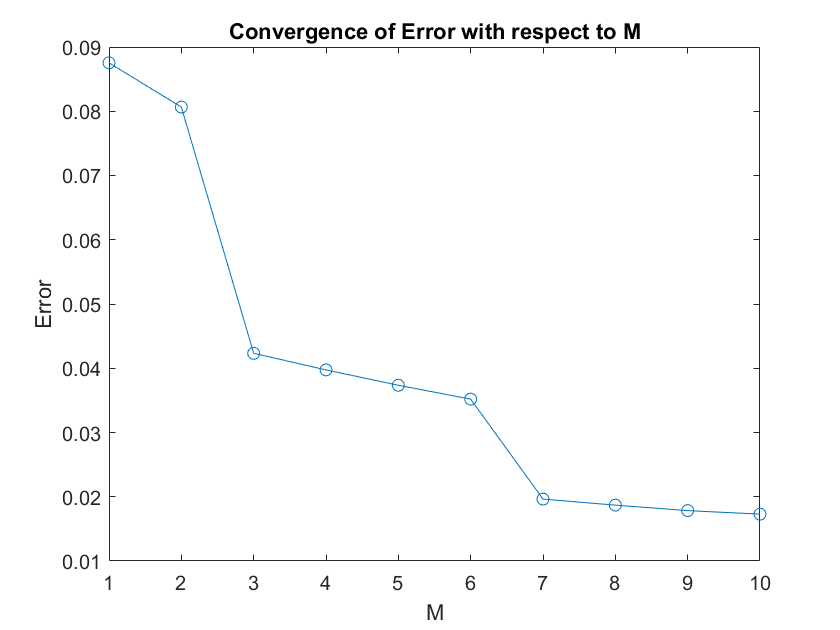
\includegraphics[width=0.6\textwidth]{pdes/fig/converge_error_m.png}
    \caption{Convergence of error with respect to $M$}
    \label{fig:converge_error_m}
\end{figure}

Figure \ref{fig:converge_error_m} shows the convergence of the error of the Finite Difference Method (FDM) solution as the number of time steps, $M$, increases.

\begin{figure}[H]
    \centering
    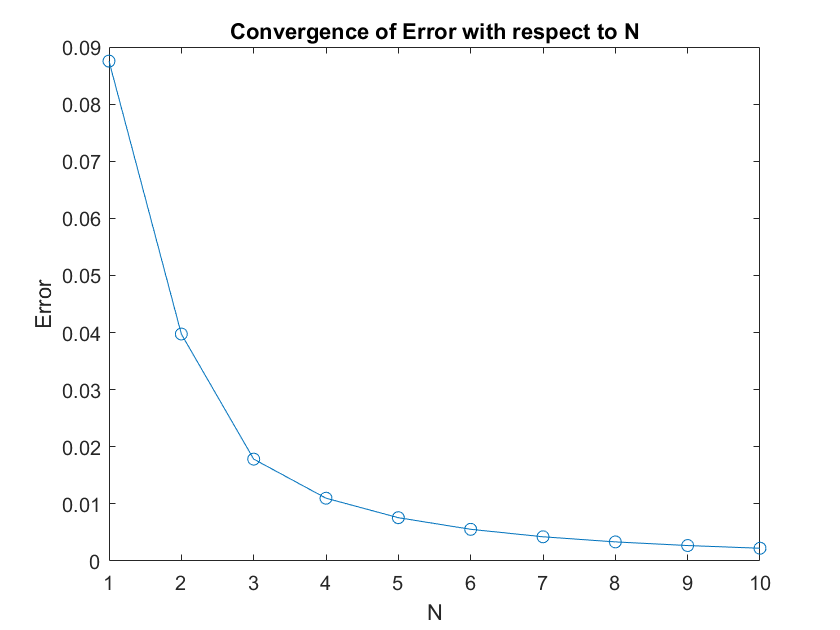
\includegraphics[width=0.6\textwidth]{pdes/fig/converge_error_n.png}
    \caption{Convergence of error with respect to $N$}
    \label{fig:converge_error_n}
\end{figure}

Figure \ref{fig:converge_error_n} illustrates the convergence of the error of the FDM solution as the number of spatial grid points, $N$, increases.

% Add MATLAB code reference
The MATLAB implementation used for generating the convergence error graphs can be found in Appendix \ref{app:convergence_of_heateq_fdm}. In addition, the code is provided in Listing \ref{lst:convergence_of_heateq_fdm} in the appendix.

\subsubsection{The Finite Element Method (FEM)}

The finite element method (FEM) is a numerical technique for solving partial differential equations (PDEs) by discretizing the domain into a collection of finite elements. The basic idea behind the FEM is to represent the solution within each element using a set of basis functions. These basis functions are typically chosen as continuous piecewise polynomials across the element boundaries. By expressing the solution as a linear combination of these basis functions, we can approximate the PDE within each element.

The variational formulation is a vital component of the finite element method. It involves transforming the PDE into an equivalent variational problem, where the goal is finding a solution that minimizes a specific function. This function is typically derived by multiplying the PDE with a test function and integrating it over the domain.

For example, let's consider the heat equation in one dimension:
\[
\partial_t u - \partial_{xx} u = f
\]
To obtain the variational formulation, we multiply the equation by a smooth test function \(v \in C^{\infty}_0(G)\) satisfying \(v(a) = v(b) = 0\), where \(G\) is the domain. 

Then, integrating the heat equation on the whole domain \(G\), we have:
\[
\int_G v \partial_t u\, dx - \int_G v \partial_{xx} u\, dx = \int_G vf\, dx
\]

Now, integrating by parts:
\[
\frac{{d}}{{dt}}\int_G u v \, dx - \left[\partial_x u (t, x) v(x) \right]_{x=a}^{x=b} + \int_G \partial_{x} u \partial_{x} v\, dx = \int_G f v\, dx
\]

Since $v$ is zero on boundaries, the second term on the left-hand side is cancelled (it equals zero).

This equation represents the variational or weak formulation of the heat equation. The goal of the finite element method is to find the solution \(u\) such that \(u(0, x) = u_0(x)\) and, for all smooth test functions \(v \in C^{\infty}_0(G)\), the following equation holds:
\[
\frac{{d}}{{dt}}\int_G u(t, x)v(x)\, dx + \int_G u'(t, x) v'(x)\, dx = \int_G f(t, x) v(x)\, dx
\]

\subsubsubsection{Galerkin Discretization}

Galerkin discretization is a key step in the finite element method (FEM), where we approximate the solution to the partial differential equation (PDE) by projecting it onto a finite-dimensional subspace. Let \(V_N\) be a finite-dimensional subspace of \(H^1_0(G)\). For each \(t \in J\), we approximate \(u(t, \cdot)\) by an element \(u_N(t, \cdot) \in V_N\):

The goal is then to find \(u_N(t, \cdot) \in V_N\) such that \(u_N(0, x) = u_{0,N}(x)\) and for all \(v_N \in V_N\), the following equation holds:

\[
\frac{{d}}{{dt}}\int_G u_N(t, x)v_N(x)\, dx + \int_G u'_{N}(t, x) v'_{N}(x)\, dx = \int_G f(t, x) v_N(x)\, dx
\]

Let \(\{b_j\}_{j=1}^N\) be a basis of \(V_N\). Then, we can express \(u_N(t, x)\) as a linear combination of basis functions:

\[
u_N(t, x) = \sum_{j=1}^N u_{N,j}(t)b_j(x)
\]

where \(\underline{u}_N(t) = (u_{N,1}(t), u_{N,2}(t), \ldots, u_{N,N}(t))^T\) is a vector of unknown functions of \(t\). Similarly, for any \(v_N \in V_N\), \(v_N(x)\) can be written as:

\[
v_N(x) = \sum_{i=1}^N v_{N,i}b_i(x)
\]

where \(v_N = (v_{N,1}, v_{N,2}, \ldots, v_{N,N})^T\) is a vector of coefficients.

\subsubsubsection{Vectorization of the equation}

Hence (we skip the argument \(x\) in \(\int_G\)):

\[
\frac{{d}}{{dt}}\int_G u_N(t)v_N + \int_G u'_{N}(t) v'_{N} = \int_G f(t)v_N, \quad \forall v_N \in V_N
\]

Which can be written as:
\[
\frac{{d}}{{dt}} \bigintssss_G \left(\sum_{j} u_{N,j}(t)b_j \right) \left( \sum_{i} v_{N,i}b_i \right) + \bigintssss_G \left( \sum_{j} u_{N,j}(t)b_{j} \right)' \left( \sum_{i} v_{N,i}b_{i} \right)' = \bigintssss_G f(t) \sum_{i} v_{N,i} b_i
\]

Simplifying further and denoting derivative with respect to time as $\dot{u}$, we have:

\[
\sum_{i} v_{N,i}\left(\sum_{j} \dot{u}_{N,j} \int_G b_j b_i + u_{N,j} \int_G b'_{j} b'_{i} - \int_G f(t) b_i\right) = 0
\]

This equation can be expressed in matrix form as:
\[
\underline{v}_N^T\left(M \underline{\dot{u_N}}(t) + A \underline{u_N} (t) - \underline{f}_N(t)\right) = 0, \quad \forall \underline{v}_N \in R^N
\]

Since it hold for all $\underline{v}_N$, expression in brackets must equal to zero, thus:

\[
M \underline{\dot{u_N}}(t) + A \underline{u_N} (t) = \underline{f}_N(t)
\]

Here \(M\) is the mass matrix with entries \(M_{ij} = \int_G b_i(x) b_j(x)\, dx \), \(A\) is the stiffness matrix with entries \(A_{ij} = \int_G b'_i(x) b'_j(x) \, dx\), \(\underline{f}_N(t)\) is the vector with entries \(f_N(t)_i = \int_G f(t)b_i\), and \(u_N(t)\) is the vector with entries \(u_{N,j}(t)\).

Therefore, we obtain the PDE:
\[
M\underline{\dot{u_N}}(t) + A \underline{u_N}(t) = \underline{f}_N(t),
\]

which is now equal to the initial heat equation \(u_N(t)\) within the finite-dimensional subspace \(V_N\):

\[
\frac{d}{{dt}}(u_N(t), v_N) + a(u_N(t), v_N) = (f(t), v_N), \quad \forall v_N \in V
\]

The Galerkin discretization is a crucial step in the finite element method as it allows us to approximate the PDE solution by solving a system of algebraic equations.

\subsubsubsection{Fully discrete scheme}

We discretize in time. To this end, write \(\underline{u}^m_N := u_N(t^m)\) and \(\underline{f}^m_N := f_N(t^m)\), where the time levels \(t^m\), \(m = 0, \ldots, M\) are as before. Proceeding exactly as in the finite difference method (FDM), the fully discrete scheme reads:

Given \(\underline{u}^0_N = (u_{0,i})^N_{i=1} \in \mathbb{R}^N\), for \(m = 0, \ldots, M-1\) find \(\underline{u}^{m+1}_N \in \mathbb{R}^N\) such that:

\[
M k^{-1} (\underline{u}^{m+1}_N - \underline{u}^m_N) + A(\theta \underline{u}^{m+1}_N + (1-\theta) \underline{u}^m_N) = \theta \underline{f}^{m+1}_N + (1-\theta) \underline{f}^m_N
\]

where \(0 \leq \theta \leq 1\) is the time discretization parameter.

The fully discrete scheme involves solving a system of algebraic equations at each time step, and it provides a numerical approximation of the PDE solution at discrete time instances within the finite-dimensional subspace \(V_N\).

\subsubsubsection{Choice of $V_N$}

The choice of the finite-dimensional subspace $V_N$ is an important aspect of Galerkin discretization. Let's define $B := M + k\theta A$, $C := M - k(1 - \theta)A$, and $\underline{F}^m_N := \theta \underline{f}^{m+1}_N + (1 - \theta) \underline{f}^m_N$. The fully discrete scheme can be written as:

\[
B \underline{u}^{m+1}_N = C \underline{u}^m_N + k \underline{F}^m_N, \quad m = 0, \ldots, M-1.
\]

To choose the space $V_N$, a common and relatively simple choice is to consider the space of piecewise linear, continuous functions. Let $\mathcal{T} := \{a = x_0 < x_1 < \ldots < x_{N+1} = b\}$ be an equidistant mesh on $G$ with $K_i := (x_{i-1}, x_i)$ (as before). We can set the following:

\[
V_N = S^1_0 := \left\{u \in C^0(G): u|_{K_i} \text{ is affine linear on } K_i \in \mathcal{T}\right\}.
\]

It's worth noting that the dimension of $V_N$ is $N$. Choosing piecewise linear functions ensures the simplicity of the basis functions and allows for a straightforward implementation of the finite element method.

A basis $\{b_i\}_{i=1}^N$ of $V_N$ is given by the so-called hat functions $b_i: [a, b] \rightarrow \mathbb{R}_{\geq 0}$, where $b_i(x) = \max\{0, 1 - h^{-1}|x - x_i|\}$ for $i = 1, \ldots, N$. 

The hat functions are defined over the interval $[a, b]$ and have a triangular shape. They take the value of 1 at the centre point $x_i$ of their corresponding subinterval $K_i$ and decrease linearly to zero as we move away from $x_i$. These basis functions capture the local behaviour of the solution within each subinterval.

For example, with equidistant mesh points $a = x_0, x_1, \ldots, x_{N+1} = b$, the basis functions are illustrated as follows:

Here is an illustration of the hat functions for equidistant mesh points:

\begin{figure}[ht]
  \centering
  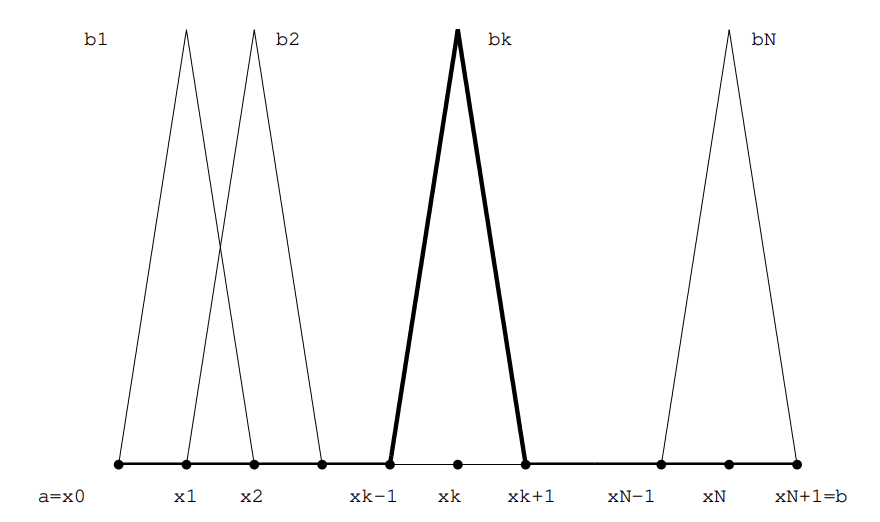
\includegraphics[width=0.6\textwidth]{pdes/fig/hat_functions.png}
  \caption{Illustration of Hat Functions}
\end{figure}

Using this basis, we can calculate the mass and stiffness matrices $M$ and $A$. For equidistant mesh points, we find:

\[
M = \frac{h}{6} \operatorname{tridiag}(1, 4, 1), \quad A = \frac{1}{h} \operatorname{tridiag}(-1, 2, -1).
\]

The mass matrix $M$ and stiffness matrix $A$ are tridiagonal matrices, where the tridiagonal structure arises from the local support of the hat functions and the properties of the integrals involved in their computation.

\subsubsection{Summary on numerical methods for PDEs}

For both Finite Difference Method (FDM) and Finite Element Method (FEM), we need to solve $M$ systems of $N$ linear equations of the form:

\[
Bu_{m+1} = Cu_m + kF_m, \quad m = 0, \ldots, M-1,
\]

where $F_m = \theta f_{m+1} + (1 - \theta)f_m$.

Let's compare the key elements of FDM and FEM:

\begin{center}
\begin{tabular}{|c|c|c|}
\hline
\textbf{Method} & \textbf{FDM} & \textbf{FEM} \\
\hline
$u_m$ & Vector of $u_{m,i} \approx u(t_m, x_i)$ & Coefficient vector of $u_N(t_m, x)$ \\
\hline
$B$ & $I + k\theta G$ & $I + k\theta M + k\theta A$ \\
\hline
$C$ & $I - k(1 - \theta) G$ & $I - k(1 - \theta) M - k(1 - \theta) A$ \\
\hline
$G | A$ & $h^{-2} \operatorname{tridiag}(-1, 2, -1)$ & $h^{-1} \operatorname{tridiag}(-1, 2, -1)$ \\
\hline
$f^m$ & $f(t_m, x_i)$ & $f^m_i = \int_G f(t_m, x) \cdot b_i(x) \, dx$ \\
\hline
\end{tabular}
\end{center}

Note, that in FDM, $f^m$ represents the discrete values of $f(t_m, x_i)$, whereas in FEM it represents the coefficient vector of $f^m_i = \int_G f(t_m, x) \cdot b_i(x) \, dx$.

Here, $G$ represents the second-order finite difference approximation of the Laplace operator, and $A$ represents the stiffness matrix. For FDM, $u_m$ represents the vector of approximate solutions at each spatial location $x_i$ and time level $t_m$. In contrast, for FEM, $u_m$ represents the coefficient vector of the approximate solution in the finite-dimensional subspace $V_N$. Finally, the matrices $B$ and $C$ are used to discretize the temporal derivative.

By solving these systems of equations, we can obtain the numerical approximations of the solution $u(t, x)$ at different time levels and spatial locations.
